\chapter{Topics}
\label{chp:topics}
Het communiceren via topics in ROS gaat via een \textit{publisher}/\textit{subscriber}-systeem. Elke node heeft de mogelijkheid om een \textit{topic} aan te maken. Nodes die informatie willen delen kunnen op een topic hun berichten \textit{publiceren}. Een node die berichten publiceert op een topic noemen we een \textit{publisher}. Nodes die deze informatie willen \textit{subscriben} zichzelf op de topic en krijgen zo de berichten binnen. Een node die berichten ontvangt van een topic noemen we een \textit{subscriber}. Het kan zijn dat een node zowel een publisher is als een subscriber. Meestal publiceert de node dan wel op een ander topic dan waarop hij is gesubscribed. Nodes kunnen ook op meerdere topics publisheren of op meerdere topics gesubscribed zijn.

Met de topic-communicatiemethode ligt het initiatief van de communicatie bij de publisher. Elke bericht dat op de topic wordt gepubliceerd wordt naar alle subscribers gestuurd. De subscribers koppelen een functie aan een topic. Bij elk bericht wordt deze functie aangeroepen om het bericht te verwerken. In figuur \ref{fig:topics} zien we dit uitgebeeld. Meerdere nodes kunnen tegelijkertijd gesubscribed zijn op een topic en meerdere nodes kunnen tegelijkertijd publishen op een topic.

\begin{figure}[h] % ’ht’ tells LaTeX to place the figure ’here’ or at the top of the page
\centering % centers the figure
\scalebox{.6}{
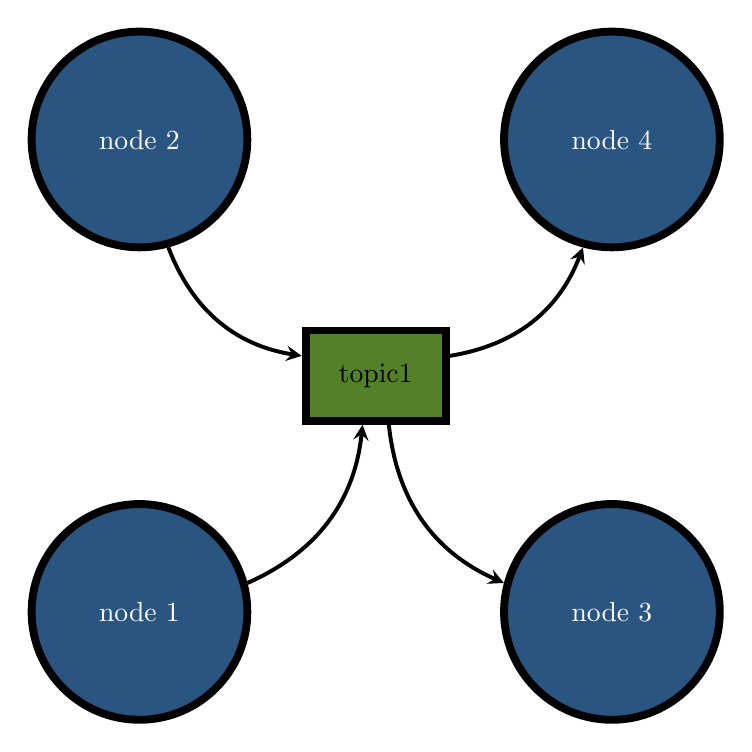
\begin{tikzpicture}[->, >=stealth, node distance=4cm, line width=1mm]
\node[circle, draw=black, fill={rgb:red,1;green,2;blue,3}, inner sep=18pt, minimum size=12pt] (A) at (0,0) {\textcolor{white}{node 1}};
\node[circle, draw=black, fill={rgb:red,1;green,2;blue,3}, inner sep=18pt, minimum size=12pt] (B) at (0,6) {\textcolor{white}{node 2}};
\node[circle, draw=black, fill={rgb:red,1;green,2;blue,3}, inner sep=18pt, minimum size=12pt] (C) at (6,0) {\textcolor{white}{node 3}};
\node[circle, draw=black, fill={rgb:red,1;green,2;blue,3}, inner sep=18pt, minimum size=12pt] (D) at (6,6) {\textcolor{white}{node 4}};
\node[rectangle, draw=black, fill={rgb:red,2;green,3;blue,1}, inner sep=12pt] (topic) at (3,3) {topic1};



\draw [->, line width=0.5mm, bend right]  (A) edge (topic)
            (B) edge (topic) 
            (topic) edge (C)
            (topic) edge (D) ;
            
        
\end{tikzpicture}
}
\caption{Een ROS topic. Node 1 en node 2 publiceren naar de topic. Node 3 en 4 zijn gesubcribed tot het topic en ontvangen daarmee de berichten van node 1 en node 2.}
\label{fig:topics}
\end{figure}

\section{Publisher code}
\label{sec:publisher}
Een node noemen we een publisher als het een membervariabele heeft van het type \textit{rclcpp::Publisher<T>}. Een rclcpp::Publisher<T> is template-class die het message-type mee moet krijgen. ROS komt met een aantal standaard messages-types\footnote{Deze moet je wel includeren!}, maar het is ook mogelijk om je eigen message-type aan te maken. We gaan dieper in op de verschillende message-types in sectie \ref{sec:message_types}. Het declareren van een rclcpp::Publisher<T> doen we binnen een node met \textit{rclcpp::Publisher<message\_type>::SharedPtr publisher\_name}. Bijvoorbeeld de publisher \textit{publisher\_} van het standaard message type String:

\begin{lstlisting}[language=C++, firstnumber=0, label={}, caption={Een publisher met het message type \textit{std\_msgs::msg::String}.}]
rclcpp::Publisher<std_msgs::msg::String>::SharedPtr publisher_;
\end{lstlisting}

\noindent Een rclcpp::Publisher kunnen we initialiseren door middel van de functie \textit{create\_publisher<T>()} die nodes erven van de superclass \textit{rclcpp::Node}. Deze functie heeft nodig: het message type, de naam van het topic en de lengte van de messages queue. Bijvoorbeeld de rclcpp::Publisher<T> \textit{publisher\_} die Strings publisht op de topic met de naam \textit{topic} en een queue van 10:
\begin{lstlisting}[language=C++, firstnumber=0, label={}]
publisher_ = this->create_publisher<std_msgs::msg::String>("topic", 10);
\end{lstlisting}

\noindent Voordat we een bericht kunnen publiceren, moeten we een message maken. Dit doen we door eerst een message te declareren en te initialiseren en vervolgens daar data aan toe te voegen. In het geval van onze standard string message gaat dat als volgt:
\begin{lstlisting}[language=C++, firstnumber=0, label={}]
auto message = std_msgs::msg::String();
message.data = "Hello, world!";
\end{lstlisting}
\noindent Het sturen van een message gaat vervolgens met de \textit{publish()}-functie van de publisher:
\begin{lstlisting}[language=C++, firstnumber=0, label={}]
publisher_->publish(message)
\end{lstlisting}

\noindent Met de boven genoemde elementen kunnen we een publisher maken. In codevoorbeelden \ref{code:hello_world_publisher_hpp}, \ref{code:hello_world_publisher_cpp} en \ref{code:hello_world_publisher_main} gebruiken we deze elementen om een publisher te maken die met behulp van een timer\footnote{Voor meer informatie over de timer zie hoofdstuk \ref{chp:ROS_nodes}.} elke 500 ms een bericht publiceert. 

\begin{lstlisting}[language=C++, caption={PublisherNode.hpp}, firstnumber=0, label={code:hello_world_publisher_hpp}]
#include "rclcpp/rclcpp.hpp"
#include "std_msgs/msg/string.hpp"

class PublisherNode : public rclcpp::Node
{
public:
  PublisherNode();
  
private:
    // function to be called by the timer.
    void timer_callback();

    // the timer:
    rclcpp::TimerBase::SharedPtr timer_;

    // publisher with message type std_msgs::msg::String :
    rclcpp::Publisher<std_msgs::msg::String>::SharedPtr publisher_;
    // variabele to count the number of messages we have sent:
    size_t count_;
};


\end{lstlisting}

\begin{lstlisting}[language=C++, caption={PublisherNode.cpp}, firstnumber=0, label={code:hello_world_publisher_cpp}]
#include "rclcpp/rclcpp.hpp"
#include "std_msgs/msg/string.hpp"
#include "PublisherNode.h"

PublisherNode::PublisherNode(): Node("PublisherNode"), count_(0){
  // initializing the publisher using the create_publisher function of the parent:
  // "topic" the name of the topic
  // 10: the size of the queue
  publisher_ = this->create_publisher<std_msgs::msg::String>("topic", 10);
  
  // initializing the timer and binding it with the function timer_callback():
  timer_ = this->create_wall_timer(
    std::chrono::milliseconds(500), 
    std::bind(&PublisherNode::timer_callback, this)
  );
}

void PublisherNode::timer_callback(){
  // a new message:
  auto message = std_msgs::msg::String();
  // adding data:
  count_++;
  message.data = "Hello, world! " + std::to_string(count_);
  // publishing the message on the topic:
  publisher_->publish(message);
}

\end{lstlisting}


\begin{lstlisting}[language=C++, caption={mainPublisher.cpp}, firstnumber=0, label={code:hello_world_publisher_main}]
#include "rclcpp/rclcpp.hpp"
#include "PublisherNode.h"

int main(int argc, char * argv[])
{
  rclcpp::init(argc, argv);
  rclcpp::spin(std::make_shared<PublisherNode>());
  rclcpp::shutdown();
  return 0;
}

\end{lstlisting}


\section{Subscriber code}
Een node noemen we een \textit{subscriber} als het een membervariabele van het type \textit{rclcpp::Subscription<T>} heeft. Een rclcpp::Subscription<T> is template-class die het message-type van de topic waarop we willen subscriben mee moet krijgen. Over message types vertellen we meer in sectie \ref{sec:message_types}. Het declareren van een publisher-variabele doen we binnen de node met \textit{rclcpp::Subscription<message\_type>::SharedPtr subscription\_name;} Bijvoorbeeld de subscription \textit{subscription\_} van het standaard message type String:
\begin{lstlisting}[language=C++, firstnumber=0, label={}]
rclcpp::Subscription<std_msgs::msg::String>::SharedPtr subscription_;
\end{lstlisting}

\noindent Een subscriber reageert altijd op elk bericht dat geplaatst wordt op het topic waartoe hij gesubscribed is. We definiëren de actie die de subscriber moet uitvoeren door bij het initialiseren van de rclcpp::Subscription<T> een functie aan de subscription te binden. Deze functie wordt vervolgens bij elk gepubliceerd bericht aangeroepen\footnote{Als een publisher een bericht publiceert roept hij eigenlijk indirect van alle subscribers een functie aan. We zeggen daarom dat het initiatief van de communicatie bij de publisher ligt. Immers de subscriber bepaalt niet zelf wanneer het een bericht van een topic afhaalt.}. Het initialiseren van een subscription doen we met de functie \textit{create\_subscription<T>()} die een node erft van de superclass \textit{rclccp::Node}. Deze functie heeft nodig: het message type, de naam van het topic, lengte van de messages queue en de functie die hij moet aanroepen als er een bericht wordt gepubliceerd. In het geval van \textit{subscription\_} in de node MyNode met het standaard message type String, de topic met de naam \textit{topic}, een queue van 10 en het aanroepen van de functie \textit{topic\_callback()} doen we dat met:
\begin{lstlisting}[language=C++, firstnumber=0, label={}]
using std::placeholders::_1;
// [...]
subscription_ = this->create_subscription<std_msgs::msg::String>(
    "topic", 10, std::bind(&MyNode::topic_callback, this, _1));
\end{lstlisting}
\noindent De \textit{std::placeholders} moeten we in de \textit{std::bind()} gebruiken omdat we een placeholder moeten geven voor de parameter (het bericht van de topic) die de functie meekrijgt\footnote{Een uitleg over \textit{std::bind} en \textit{std::placeholders} kan men vinden op: \url{https://www.youtube.com/watch?v=JtUZmkvroKg}}.

Als er een bericht wordt gepubliceerd dan wordt de functie aangeroepen met als parameter de message. Hieronder een voorbeeld van functie die een message ontvangt en deze print via de logger:

\begin{lstlisting}[language=C++, firstnumber=0, label={}]
void topic_callback(const std_msgs::msg::String::SharedPtr msg) const{
    RCLCPP_INFO(this->get_logger(), "I heard: '%s'", msg->data.c_str());
}
\end{lstlisting}

\noindent Met de boven genoemde elementen kunnen we een subscriber maken. In codevoorbeelden \ref{code:hello_world_subscriber_hpp}, \ref{code:hello_world_subscriber_cpp} en \ref{code:hello_world_subscriber_main} gebruiken we deze elementen om een subscriber te maken die elke keer als er een bericht wordt gepubliceerd op de topic met de naam \textit{topic} de functie \textit{topic\_callback()} aanroept.

\begin{lstlisting}[language=C++, caption={Subscriber.hpp}, firstnumber=0, label={code:hello_world_subscriber_hpp}]
#include "rclcpp/rclcpp.hpp"
#include "std_msgs/msg/string.hpp"

class SubscriberNode : public rclcpp::Node
{
public:
    SubscriberNode();

private:
    // the function called everytime we receive a message from the topic:
    void topic_callback(const std_msgs::msg::String::SharedPtr msg) const;

    // the subscription:
    rclcpp::Subscription<std_msgs::msg::String>::SharedPtr subscription_;
};
\end{lstlisting}


\begin{lstlisting}[language=C++, caption={Subscriber.cpp}, firstnumber=0, label={code:hello_world_subscriber_cpp}]
#include "rclcpp/rclcpp.hpp"
#include "std_msgs/msg/string.hpp"
#include "SubscriberNode.h"

using std::placeholders::_1;

SubscriberNode::SubscriberNode(): Node("minimal_subscriber"){
  // initialize the subscription with:
  // "topic" name of the topic
  // 10: size of the queue buffer for backup
  // binding the function topic_callback()
  // with std::placeholders::_1 we place a placeholder for the 
  // function parameter (the message from the topic)
  subscription_ = this->create_subscription<std_msgs::msg::String>(
    "topic", 10, std::bind(&SubscriberNode::topic_callback, this, _1));
}


void SubscriberNode::topic_callback(const std_msgs::msg::String::SharedPtr msg) const
{
  RCLCPP_INFO(this->get_logger(), "I heard: '%s'", msg->data.c_str());
}
\end{lstlisting}


\begin{lstlisting}[language=C++, caption={mainSubscriber.cpp}, firstnumber=0, label={code:hello_world_subscriber_main}]
#include "rclcpp/rclcpp.hpp"
#include "SubscriberNode.h"

int main(int argc, char * argv[])
{
  rclcpp::init(argc, argv);
  rclcpp::spin(std::make_shared<SubscriberNode>());
  rclcpp::shutdown();
  return 0;
}
\end{lstlisting}

\section{Message types}
\label{sec:message_types}
ROS komt met een groot aantal build-in message types\footnote{Voor de complete lijst: \url{https://index.ros.org/p/std_msgs/}}. Je code krijgt toegang hier toe door \textit{std\_msgs}\footnote{Of specifieker als je een string-message wil: \textit{std\_msgs/msg/string.hpp}} te includen en toe te voegen aan je dependencies in package.xml\footnote{\textit{<depend>std\_msgs</depend>}} en CMakeLists.txt\footnote{\textit{find\_package(std\_msgs REQUIRED)} plus toevoegen aan \textit{ament\_target\_dependencies()}}.
Het is ook mogelijk om zelf message types te maken. Dit doe je door een \textit{.msg}-bestand te maken. \textit{.msg}-bestanden zijn te gebruiken als ze binnen je package staan, maar het is ook mogelijk om gebruik te maken van een \textit{.msg}-bestand uit een andere package. Een conventie is om een aparte package te maken met alle message-types. Andere conventies geven juist weer voorkeur aan het plaatsen van de message-types binnen de packages die ze gebruiken. Waar de message-types staan is dus onderhevig aan de voorkeur van de programmeur/het team. In de codevoorbeelden die komen bij deze cursus staan voorbeelden met custom messages binnen het buiten de package. Meer informatie over hoe je zelf een message type maakt kan je vinden op:
\begin{center}
    {\footnotesize \url{https://index.ros.org/doc/ros2/Tutorials/Custom-ROS2-Interfaces/}}\\
    en extra verdieping: \\
    {\footnotesize \url{https://index.ros.org/doc/ros2/Tutorials/Single-Package-Define-And-Use-Interface/}}
\end{center}
\noindent \textbf{Let op:} Bij het maken van een custom message type is het verplicht in de naamgeving PascalCase\footnote{zie \url{https://nl.wikipedia.org/wiki/CamelCase}} te gebruiken. ROS zet de custom message om naar een \textit{.hpp}-bestand met de naam in snake\_case \footnote{zie: \url{https://en.wikipedia.org/wiki/Snake_case}}, waarbij tussen elke kleine letter en hoofdletter van de PascalCase naamgeving nu een onderstrepingsteken (\_)\footnote{ook wel bekent als \textit{underscore}. Zie \url{https://nl.wikipedia.org/wiki/Underscore}} staat. Bijvoorbeeld de custom message \textit{MyCustomMessage.msg} wordt geïncludeerd met \textit{\#include "path/to/folder/my\_custom\_message.hpp"}.

\section{Publisher revisited}
In sectie \ref{sec:publisher} hebben we een publisher gemaakt die om gezette intervallen een bericht stuurt. Hiervoor hebben we gebruik gemaakt van een \textit{wall timer} die steeds een callback\footnote{Een callback is een bericht/functieaanroep die een node moet afhandelen. Bijvoorbeeld in de publisher van sectie \ref{sec:publisher} is dit de de wall timer die afloopt en \textit{timer\_callback()} aanroept en bij de subscriber in dit hoofdstuk is dat het ontvangen van een bericht van de topic en daarmee de aanroep van de functie \textit{topic\_callback()}. Om callbacks te ontvangen/af te handelen moet een node aan het spinnen zijn.} doet naar een functie van de node. Dit is een logische implementatie voor bijvoorbeeld een sensornode die elke 500 miliseconden de waarde van de sensor uitleest en deze publiceert.

Er zijn echter ook systemen die niet elk interval iets moeten publiceren, maar constant aan het werk zijn en direct moeten publiceren als ze iets detecteren. Het is daarom belangrijk te realiseren dat het spinnen\footnote{De functie \textit{rclcpp::spin()}; al zijn er ook andere opties hiervoor. Zie: \url{https://docs.ros2.org/foxy/api/rclpy/api/init_shutdown.html} en \url{https://docs.ros2.org/foxy/api/rclpy/api/execution_and_callbacks.html}.} alleen nodig is als de node callback's moet kunnen ontvangen. Voor het publiceren is het niet nodig dat de node aan het spinnen is. Codevoorbeeld \ref{code:publising_main} geeft ons een voorbeeld hiervan. De main-functie in het codevoorbeeld maakt door middel van een node een publisher en gebruikt deze om 10 berichten te sturen.

\begin{lstlisting}[language=C++, caption={publishingMain.cpp; zonder node-subclass en zonder \textit{rclcpp::spin()}}, firstnumber=0, label={code:publising_main}]
#include "rclcpp/rclcpp.hpp"
#include "std_msgs::msg::String>("

int main(int argc, char * argv[])
{
    rclcpp::init(argc, argv);
    auto node = std::make_shared<rclcpp::Node>("my_node");
    auto pub = node->create_publisher<std_msgs::msg::String>(>("topic", 10);

    auto message = std_msgs::msg::String>(();
    int count = 0;
    
    for(int i=0; i<10; i++){
        int count++;
        message.data = "Hello, world! " + std::to_string(count);
        pub->publish(message);
        
        for(int j=0; j<1000000000; j++){} // wait some time
    }

    return 0;
}
\end{lstlisting}

\noindent Het is natuurlijk ook mogelijk om een node-class te maken die publiceert zonder dat hij spint. in codevoorbeelden \ref{code:hello_world_publisher_hpp_no_spinning}, \ref{code:hello_world_publisher_cpp_no_spinning} en \ref{code:hello_world_publisher_main_no_spinning} zien we een custom publishing node die wel publisheert, maar niet spint.

%YYYYYYYYYYYY newpage
\newpage %<- !!!!!!!!!!!!!!!!!!! <-
%YYYYYYYYYYYYY newpage

\begin{lstlisting}[language=C++, caption={PublisherNode.hpp; zonder een wall timer.}, firstnumber=0, label={code:hello_world_publisher_hpp_no_spinning}]
#include "rclcpp/rclcpp.hpp"
#include "std_msgs/msg/string.hpp"

class PublisherNode : public rclcpp::Node
{
public:
    PublisherNode();
  
private:.
    void publishHelloWorld(const int & n);

    // publisher with message type std_msgs::msg::String :
    rclcpp::Publisher<std_msgs::msg::String>::SharedPtr publisher_;
};


\end{lstlisting}

\begin{lstlisting}[language=C++, caption={PublisherNode.cpp; zonder een wall timer.}, firstnumber=0, label={code:hello_world_publisher_cpp_no_spinning}]
#include "rclcpp/rclcpp.hpp"
#include "std_msgs/msg/string.hpp"
#include "PublisherNode.h"

PublisherNode::PublisherNode(): Node("PublisherNode"){
  publisher_ = this->create_publisher<std_msgs::msg::String>("topic", 10);
}

void PublisherNode::publishHelloWorld(const int & n){

    auto message = std_msgs::msg::String();
    int count = 0;
    
    for(int i=0; i<n; i++){
        int count++;
        message.data = "Hello, world! " + std::to_string(count);
        pub->publish(message);
        
        for(int j=0; j<1000000000; j++){} // wait some time
    }
}

\end{lstlisting}


\begin{lstlisting}[language=C++, caption={mainPublisher.cpp; zonder rclcpp::spin()}, firstnumber=0, label={code:hello_world_publisher_main_no_spinning}]
#include "rclcpp/rclcpp.hpp"
#include "PublisherNode.h"

int main(int argc, char * argv[])
{
  rclcpp::init(argc, argv);
  auto node = PublisherNode();
  node.publishHelloWorld(10);
  return 0;
}

\end{lstlisting}